\documentclass[a4paper,master=mai,masteroption=ecs,english]{kulemt}
\usepackage{multibib}
\newcites{lrucs}{ }
\setup{
  inputenc=utf8,
  title={Neural network calibration for DeepProbLog},
  author={Joshua Schroijen},
  promotor={Prof.\,Luc D	e Raedt},
  assessor={},
  assistant={Dr.\,Ir.\,Robin Manhaeve}
}
\setup{font=lm}
\begin{document}
\begin{preface}
I would like to sincerely thank my academic supervisor, Dr. Ir. Luc De Raedt and my daily supervisor, Dr. Ir. Robin Manhaeve, for all their patient help and insightful input in the process of creating this work. \par
I would also like to thank my family in general and my partner in particular. This thesis was written under personally challenging circumstances and I genuinely could not have completed it without their day to day support and encouragement.
\end{preface}
\tableofcontents*
\begin{abstract}
In recent years, the field of machine learning effectively leveraged increased computing power. Through increasingly complex topologies, performance breakthroughs were achieved in image classification, machine translation, text and image generation and other applications. However, it was unfortunately observed that this generally came at a large expense of network calibration or the confidence networks have in their predictions. This presents a dilemma to the subfield of neuro-symbolic integration for probabilistic inference, where ideally neural networks' excellent learning capabilities are combined with necessarily sound calibration. We implement temperature scaling calibration schemes in representative applications of the DeepProbLog probabilistic logic programming language and measure differences in model performance. We conclude whether model calibration is necessary or beneficial in this context.
\end{abstract}
\listoffiguresandtables
\chapter{List of Abbreviations and Symbols}
\section*{Abbreviations}
\begin{flushleft}
\renewcommand{\arraystretch}{1.1}
\begin{tabularx}{\textwidth}{@{}p{12mm}X@{}}
GOFAI & Good Old Fashioned AI \\
KB & Knowledge Base \\
SRL & Statistical Relational Learning \\
PLP & Probabilistic Logic Programming \\
nAD & Neural annotated disjunction \\
RD & Reliability diagram \\
ECE & Expected Calibration Error \\
MCE & Maximum Calibration Error \\
NLL & Negative log-likelihood \\
BBQ & Bayesian binning into quantiles
\end{tabularx}
\end{flushleft}
\section*{Symbols}
\mainmatter
\chapter{Introduction}
In \cite{haugeland1989artificial}, Haugeland introduced a popular categorization of AI methodologies: symbolic and sub-symbolic AI. He simultaneously coined the term Good Old Fashioned AI (GOFAI) for the former. Symbolic AI systems work with knowledge explicitly declared by humans using symbols in knowledge bases (KBs). Manipulation rules are applied to the elements of this KB to answer queries or solve problems. Sub-symbolic methodologies do not require humans to explicitly encode knowledge, but rather infer model structure and/or parameters from data in some way. Logic programming is a prominent form of symbolic AI while neural networks are renowned sub-symbolic AI models. \par
\cite{lighthill1973ai} infamously concluded that none of the discoveries made by 1973 in symbolic AI had produced the promised impact. After its publication, the UK government cut funding for all but two of its universities' AI research groups in a move that is widely regarded as the start of AI's first winter. Disillusionment with machine translation in particular was great. Interest in symbolic AI resurged in the 80s with expert systems. But when expert systems were found to lack common sense to a problematic degree, the second AI winter began and symbolic AI's reputation suffered damage lasting to today. Ever more researchers agreed with Lighthill's diagnosis and conclusions: symbolic AI suffered from a severe combinatorial complexity explosion problem both in KB creation and use due to its heavy reliance on search algorithms and researchers' failure to mitigate this issue meant symbolic AI was unlikely to ever scale up to real world problems. After the second AI winter, sub-symbolic AI methods would dominate new AI efforts and breakthroughs. In contrast to symbolic approaches, sub-symbolic methods had a hard and slow start but manage to tackle industrial challenges such as image classification, text generation and machine translation now after this decade's deep learning revolution. They have truly become excellent go-to methods for regression and classification problems. \par
However, in recent years researchers have come to reappreciate symbolic methods, as while they might not scale enough on their own they still achieved and offer several unique and powerful features and properties. For all the leaps forward in sub-symbolic AI, the incorporation of a priori knowledge is still very difficult and the ability to actively reason and explain this reasoning is still mostly missing. We should thus see symbolic and sub-subsymbolic methods not as competing with but possibly complementary to one another. Many works such as \cite{garcez2015neural} even already argue that combining symbolic and sub-symbolic ideas is a necessity to build AI that can effectively learn and reason. This view led to the subfield of neuro-symbolic integration. Many means of integration are being explored, but we are particularly interested in doing so through extending the paradigm of logic programming since it would aid generally interesting fields KU Leuven's DTAI Research Group (for whom this thesis is written) is working in like statistical relational learning (SRL) and probabilistic inference. \cite{ng1992probabilistic} already considered probabilistic logic programming (PLP), which could be a powerful SRL framework, in 1992. \cite{fierens2015inference} also discusses how, because both PLP and probabilistic inference can be reduced to weighted \#SAT PLP is attractive for the latter given the potential ease of modelling problems in it. \par
Logic programs are KBs containing logical facts and rules (also known as predicates) declared in a formal logic programming language such as Prolog. To execute a logic program is to query the KB with a logical statement that might contain variables. A logic program then returns whether or not the logical statement is true and optionally the set of variable assignments that make it so. Logic programs ideally have no procedural meaning but do in practice, where one has to consider the query evaluation algorithm used (such as Prolog's unification) to ensure the KB is written in a way that gives the correct results. \par
There are some extensions to logic programming which add additional semantics to facts, rules and query results. In PLP, facts and rules are assigned probabilities of holding and query results are extended by the probability of returned models. Our extension of interest here is the integration of neural networks in PLPs. \cite{manhaeve2018deepproblog} showed such an extension of ProbLog (a PLP language based on Prolog developed by KU Leuven's DTAI Research Group) in 2018 called DeepProbLog. DeepProblog introduces neural predicates. Neural predicates take an input and an output variable. The output variable will be unified with the underlying neural network's output given the input variable, which should be instantiated when the predicate is evaluated. These underlying neural networks are declared in the form of a so called neural annotated disjunction (nAD). When the parameters (such as unknown probabilities) of the DeepProbLog program are determined, they will be trained based on an externally supplied dataset. \par
DeepProbLog still faces a major challenge, though. While the use of deeper architectures has dramatically improved classification and regression performances, as \cite{guo2017calibration} points out this has come at the cost of model callibration. A model's callibration is its ability to associate probabilities to its predictions that match the ground truth likelihoods of it being correct. Good callibration is naturally crucial when incorporating neural networks into PLP (or other probabilistic models for that matter). In the case of DeepProbLog we are indeed primarily interested in the neural networks producing accurate probabiltiy distributions over target space given the input rather than concrete deterministic predictions, since we are performing probabilistic rather than deterministic queries. \par
\chapter{Literature review}
\section{Review of the calibration problem and calibration methods}
In this section we will summarize \cite{guo2017calibration}'s findings and propositions on the topic of neural network calibration.

\subsection{The general problem of neural network model calibration degradation}
\cite{guo2017calibration} discovered that they could not confirm \cite{niculescu2005predicting}'s observation that neural networks (for binary classification) were typically well-calibrated for the latest generation of deep neural network models. \cite{lecun1998gradient}'s 5-layer LeNet was compared to \cite{he2016deep}'s 110 layer ResNet on the CIFAR-100 dataset. This comparison is visualized in figure \ref{fig:lenet_vs_resnet_calibration_guo_et_al}, where the top row shows prediction confidence histograms and the bottom row shows reliability diagrams (RDs). RDs show a model's accuracy as a function of its confidence. A perfectly callibrated model has a 45° angled line, i.e. the identity function, as its RD. Figure \ref{fig:lenet_vs_resnet_calibration_guo_et_al} shows a striking overconfidence of the ResNet on CIFAR-100 while showing the LeNet has an almost perfect RD on it. \cite{guo2017calibration} thus proposes that the modern ResNet has gained in accuracy over the older LeNet by, through some mechanism, sacrificing calibration. Through abductive reasoning \cite{guo2017calibration} hypothesizes and substantiates that this is a general and explainable evolutionary trend in artificial neural network R\&D that one could call calibration degradation. 

\begin{figure}[htbp!]
  \centering
  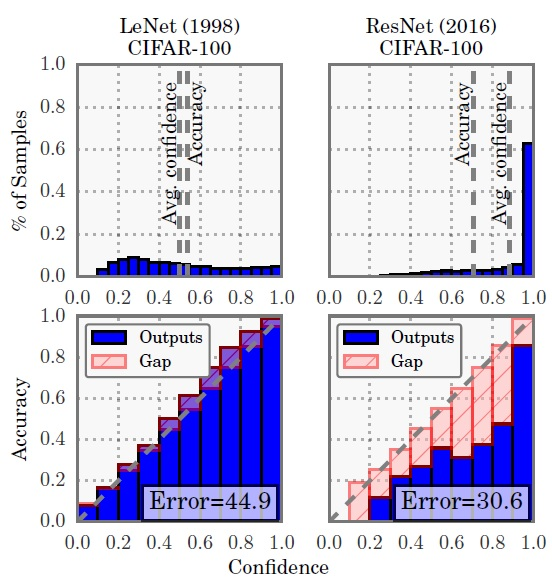
\includegraphics[width=0.6\linewidth]{images/lenet_vs_resnet_calibration_guo_et_al.jpg}
  \caption[5-layer LeNet's vs. 110-layer ResNet's calibration.]{5-layer LeNet (left) vs. 110-layer ResNet (right) calibration.}
  \label{fig:lenet_vs_resnet_calibration_guo_et_al}
  \source{\cite{guo2017calibration}}
\end{figure}
\newpage

\subsection{Formal calibration definitions and metrics}
\cite{guo2017calibration} provide a rigorous definition of and enumerate several metrics for the calibration of supervised multiclass classification.

\subsubsection{Notation and the formal perfect calibration definition}
The input $X \in \mathcal{X}$ and label $Y \in \mathcal{Y}=\{1, \ldots, K\}$ are random variables that follow a ground truth joint distribution $\pi(X, Y)=$ $\pi(Y \mid X) \pi(X)$. Let $h$ be a neural network with $h(X)=$ $(\hat{Y}, \hat{P})$, where $\hat{Y}$ is a class prediction and $\hat{P}$ is its confidence or self-estimated probability of correctness. Neural network $h$ is theoretically defined as perfectly calibrated if and only if equation \ref{eqn:perfect_calibration_in_theory} holds over the ground truth joint distribution $\pi(X, Y)$.
\begin{equation}
  \label{eqn:perfect_calibration_in_theory}
  \mathbb{P}(\hat{Y}=Y \mid \hat{P}=p)=p, \quad \forall p \in[0,1]
\end{equation}

Equation \ref{eqn:perfect_calibration_in_theory} is not practically applicable: $p$ is a continuous variable, therefore equation \ref{eqn:perfect_calibration_in_theory}'s satisfaction cannot be checked in finite time. Equation \ref{eqn:perfect_calibration_in_practice} can instead be used in practice. It is a binning method where predictions are grouped into $M$ equally sized bins over the interval $\interval{0}{1}$ based on their associated confidence.

\begin{align}
  \label{eqn:perfect_calibration_in_practice}
  \operatorname{acc}\left(B_{m}\right) &= \operatorname{conf}\left(B_{m}\right), \quad \forall m \in[0,M] \\ \nonumber
  \text{where}~\operatorname{acc}\left(B_{m}\right) &= \frac{1}{\left|B_{m}\right|} \sum_{i \in B_{m}} \mathbf{1}\left(\hat{y}_{i}=y_{i}\right), \\ \nonumber
  \operatorname{conf}\left(B_{m}\right) &= \frac{1}{\left|B_{m}\right|} \sum_{i \in B_{m}} \hat{p}_{i}, \\ \nonumber
  B_{m} &= \parbox[t]{8cm}{\raggedright The set of indices of samples whose prediction confidence falls into the interval $I_{m}$,} \\ \nonumber
  I_{m} &= \left[\frac{m-1}{M}, \frac{m}{M}\right], \\ \nonumber
  \hat{y}_{i} &= \text{Predicted class label of sample $i$}, \\ \nonumber
  y_{i} &= \text{True class label of sample $i$}, \\ \nonumber
  \hat{p}_{i} &= \text{Confidence of the class prediction of sample $i$}
\end{align}

$\operatorname{acc}\left(B_{m}\right)$ is an unbiased and consistent estimator of $\mathbb{P}\left(\hat{Y}=Y \mid \hat{P} \in I_{m}\right)$ by basic probability theory.

\subsubsection{Calibration metrics}
To make the criterion of perfect calibration, which is a goal that can rarely be reached in practice, useful we need to combine it with a quantitative measure of how close a model is to meeting it. Such a measure then allows us to bring a model ever closer to being perfectly calibrated instead of only to determine whether or not it is so. Three main metrics are layed out by \cite{guo2017calibration} and discussed here. We will call these metrics miscalibration metrics.

\paragraph{Expected Calibration Error (ECE)}
The expected calibration error (ECE), defined by equation \ref{eqn:ece_theoretical}, quantifies miscalibration as the expected absolute difference between the true accuracy of the model given its probabilistic confidence and its probabilistic confidence.
\begin{equation}
  \label{eqn:ece_theoretical}
  \mathrm{ECE}=\underset{\hat{P}}{\mathbb{E}}[|\mathbb{P}(\hat{Y}=Y \mid \hat{P}=p)-p|]
\end{equation}
Equation \ref{eqn:ece_theoretical} cannot be evaluated in practice because $\hat{P}$ is a continuous variable. Therefore equation \ref{eqn:ece_practical}, an approximation-by-binning method similar to equation \ref{eqn:perfect_calibration_in_practice} is used in practice.
\begin{equation}
  \label{eqn:ece_practical}
  \mathrm{ECE}=\sum_{m=1}^{M} \frac{\left|B_{m}\right|}{n}\left|\operatorname{acc}\left(B_{m}\right)-\operatorname{conf}\left(B_{m}\right)\right| \text {, }
\end{equation}
The expected calibration error metric is appropriate for use in model calibration optimization if calibration outliers are acceptable. ECE is ideally 0.

\paragraph{Maximum Calibration Error (MCE)}
The maximum calibration error (MCE), defined by equation \ref{eqn:mce_theoretical}, quantifies miscalibration as the maximum absolute difference between the true accuracy of the model given its probabilistic confidence and its probabilistic confidence.
\begin{equation}
  \label{eqn:mce_theoretical}
  \mathrm{MCE}=\max _{p \in[0,1]}|\mathbb{P}(\hat{Y}=Y \mid \hat{P}=p)-p| \text {. }
\end{equation}
Equation \ref{eqn:mce_theoretical} cannot be evaluated in practice because $\hat{P}$ is a continuous variable. Therefore equation \ref{eqn:mce_practical}, an approximation-by-binning method similar to equation \ref{eqn:perfect_calibration_in_practice} is used in practice.
\begin{equation}
  \label{eqn:mce_practical}
  \mathrm{MCE}=\max _{m \in\{1, \ldots, M\}}\left|\operatorname{acc}\left(B_{m}\right)-\operatorname{conf}\left(B_{m}\right)\right|
\end{equation}
The maximum calibration error metric is appropriate for use in model calibration optimization if calibration outliers are problematic. MCE is ideally 0.

\paragraph{Negative log-likelihood (NLL)}
Negative log-likelihood (also commonly known as cross-entropy loss in deep learning) $\mathcal{L}$ is a standard measure of probabilistic model fit. Equation \ref{eqn:nll_theoretical} gives its definition.

\begin{align}
  \label{eqn:nll_theoretical}
  \mathcal{L} &= -\sum_{i=1}^{n} \log \left(\hat{\pi}\left(y_{i} \mid \mathbf{x}_{i}\right)\right) \\ \nonumber
  \text{where}~\hat{\pi}(Y \mid X) &= \text{The probabilistic model under evaluation,} \\ \nonumber
  n &= \text{The number of samples}
\end{align}
Minimizing equation \ref{eqn:nll_theoretical} brings $\hat{\pi}(Y \mid X)$ ever closer to the true probability distribution. If negative log-likelihood is 0, $\hat{\pi}(Y \mid X)$ is the ground truth probability distribution. We do not use negative log-likelihood in practice to calibrate deep learning models because in this context \cite{guo2017calibration} show that it is too susceptible to overfitting.

\subsection{Calibration methods}
\cite{guo2017calibration} provide and compare several calibration methods we will discuss here.

\subsubsection{Histogram binning}
Histogram binning is a non-parametric calibration method where all uncalibrated prediction confidences $\hat{p}_{i}$ of the dataset are divided into bins $B_{1}, \ldots, B_{M}$. Each bin is assigned a calibrated prediction confidence $\theta_{m}$ such that if $\hat{p}_{i}$ is assigned to bin $B_{m}$, then $\hat{q}_{i}=\theta_{m}$ where $\hat{q}_{i}$ stands for sample $i$'s calibrated prediction confidence. The $\theta_{m}$'s are chosen to minimize the bin-wise squared loss as defined by equation \ref{eqn:histogram_binning} in the case of binary classification.
\begin{align}
  \label{eqn:histogram_binning}
  \min_{\theta_{1}, \ldots, \theta_{M}} &\sum_{m=1}^{M} \sum_{i=1}^{n} \mathbf{1}\left(a_{m} \leq \hat{p}_{i}<a_{m+1}\right)\left(\theta_{m}-y_{i}\right)^{2} \\ \nonumber
  \text{where}~\hat{p}_{i} &= \text{The uncalibrated probability of sample $i$ being positive (1)}
  M &= \text{The number of bins}, \\ \nonumber
  n &= \text{The number of samples}, \\ \nonumber
  1 &= \text{The indicator function}, \\ \nonumber
  0=a_{1} \leq a_{2} \leq \ldots \leq a_{M+1}=1 &= \parbox[t]{5cm}{The boundaries of bin $B_{m}$ defined by the interval $\left(a_{m}, a_{m+1}\right]$,} \\ \nonumber
  \theta_{m} &= \parbox[t]{5cm}{The calibrated prediction confidence associated with bin $m$,} \\ \nonumber
  y_{i} &= \parbox[t]{5cm}{Sample $i$'s true class, either positive (1) or negative (0)}
\end{align}
Typically the bins are either made equally long or sized to equalize the number of samples they contain.
Given fixed bin boundaries, the solution to equation \ref{eqn:histogram_binning} is to let $\theta_{m}$ be equal to the average number of positive-class samples in bin $B_{m}$.

\subsubsection{Isotonic regression}
Isotonic regression is a generalization of histogram binning where not only the calibrated prediction confidences of each bin but also the bin boundaries are optimized, as defined by equation \ref{eqn:isotonic_regression} in the case of binary classification.
\begin{align}
  \label{eqn:isotonic_regression}
  \min _{
    \begin{array}{c}
      M \\
	  \genfrac{}{}{0pt}{}{\theta_{1}, \ldots, \theta_{M}}{a_{1}, \ldots, a_{M+1}}
    \end{array}
  } & \sum_{m = 1}^{M} \sum_{i = 1}^{n} 1\left(a_{m} \leq \hat{p}_{i} < a_{m + 1}\right)\left(\theta_{m} - y_{i}\right)^{2} \\ \nonumber
  \text{ subject to } & 0 = a_{1} \leq a_{2} \leq \ldots \leq a_{M + 1}=1, \\
  & \theta_{1} \leq \theta_{2} \leq \ldots \leq \theta_{M}. \\ \nonumber
  \text{where}~\hat{p}_{i} &= \text{The uncalibrated probability of sample $i$ being positive (1)}
  M &= \text{The number of bins}, \\ \nonumber
  n &= \text{The number of samples}, \\ \nonumber
  1 &= \text{The indicator function}, \\ \nonumber
  0=a_{1} \leq a_{2} \leq \ldots \leq a_{M+1}=1 &= \parbox[t]{5cm}{The boundaries of bin $B_{m}$ defined by the interval $\left(a_{m}, a_{m+1}\right]$,} \\ \nonumber
  \theta_{m} &= \parbox[t]{5cm}{The calibrated prediction confidence associated with bin $m$,} \\ \nonumber
  y_{i} &= \parbox[t]{5cm}{Sample $i$'s true class, either positive (1) or negative (0)}
\end{align}

\subsubsection{Bayesian binning into quantiles (BBQ)}
Bayesian binning into quantiles (BBQ) is a Bayesian maximum a posteriori (MAP) calibrated probability estimation method that can be seen as a variation on histogram binning. Its basis is marginalization over the space of all possible binning schemes $\mathcal{S}$. We define a binning scheme $s$ as a pair $(M, \mathcal{I})$ where $M$ is the number of bins, and $\mathcal{I}$ is a corresponding partitioning of $[0,1]$ into $M$ disjoint intervals with boundaries $0=a_{1} \leq a_{2} \leq \ldots \leq a_{M+1}=1$. A binning scheme has parameters $\theta_{1}, \ldots, \theta_{M}$ defining a generative model for data on it. Equation \ref{eqn:bbq_pq} shows how a probability distribution of the calibrated confidence $\hat{q}$ conditioned on the data ($D$) and the uncalibrated confidence $\hat{p}$ can be defined as a marginalization over the space of all possible binning schemes. Equation \ref{eqn:bbq_pq_in_terms_of_s} shows

\begin{align}
\label{eqn:bbq_pq}
\mathbb{P}\left(\hat{q} \mid \hat{p}, D\right) &= \sum_{s \in \mathcal{S}} \mathbb{P}\left(\hat{q}, S=s \mid \hat{p}, D\right) \\
\label{eqn:bbq_pq_in_terms_of_s}
&= \sum_{s \in \mathcal{S}} \mathbb{P}\left(\hat{q} \mid \hat{p}, S=s, D\right) \mathbb{P}(S=s \mid D)
\end{align}

Using a uniform prior, the weight $\mathbb{P}(S=s \mid D)$ from equation \ref{eqn:bbq_pq_in_terms_of_s} can be derived using Bayes' rule:
\begin{equation}
\label{eqn:ps_given_d}
\mathbb{P}(S=s \mid D)=\frac{\mathbb{P}(D \mid S=s)}{\sum_{s^{\prime} \in \mathcal{S}} \mathbb{P}\left(D \mid S=s^{\prime}\right)}.
\end{equation}
By viewing parameters $\theta_{1}, \ldots, \theta_{M}$ as parameters of $M$ independent binomial distributions and by placing Beta priors on them, we can obtain a closed form expression for the marginal likelihood $\mathbb{P}(D \mid S=s)$. This allows us to backtrack through equations \ref{eqn:ps_given_d}, \ref{eqn:bbq_pq_in_terms_of_s} and \ref{eqn:bbq_pq} to finally compute $\mathbb{P}\left(\hat{q} \mid \hat{p}, D\right)$ for any test input.

Using equation \ref{eqn:bbq_pq} to \ref{eqn:ps_given_d}, we can use equation \ref{eqn:bbq_pq_argmax} to determine the calibrated confidence of the model given the data and its uncalibrated confidence. This is Bayesian binning into quantiles.
\begin{equation}
\label{eqn:bbq_pq_argmax}
\hat{q} = \argmax_{\hat{q}} \mathbb{P}\left(\hat{q} \mid \hat{p}, D\right)
\end{equation}

\subsubsection{Platt and temperature scaling}
\subsubsection{Comparison}
  
\begin{table}
  \centering
  \resizebox{\linewidth}{!}{
    \begin{tabular}{ *{9}{c} }
      \hline
      Dataset & Model & Uncalibrated & Hist. Binning & Isotonic & BBQ & Temp. Scaling & Vector Scaling & Matrix Scaling \\
      \hline
      Birds & ResNet 50 & $9.19\%$ & $4.34\%$ & $5.22\%$ & $4.12\%$ & $1.85\%$ & $3.0\%$ & $21.13\%$ \\
      Cars & ResNet 50 & $4.3\%$ & $1.74\%$ & $4.29\%$ & $1.84\%$ & $2.35\%$ & $2.37\%$ & $10.5\%$ \\
      CIFAR-10 & ResNet 110 & $4.6\%$ & $0.58\%$ & $0.81\%$ & $0.54\%$ & $0.83\%$ & $0.88\%$ & $1.0\%$ \\
      CIFAR-10 & ResNet 110 (SD) & $4.12\%$ & $0.67\%$ & $1.11\%$ & $0.9\%$ & $0.6\%$ & $0.64\%$ & $0.72\%$ \\
      CIFAR-10 & Wide ResNet 32 & $4.52\%$ & $0.72\%$ & $1.08\%$ & $0.74\%$ & $0.54\%$ & $0.6\%$ & $0.72\%$ \\
      CIFAR-10 & DenseNet 40 & $3.28\%$ & $0.44\%$ & $0.61\%$ & $0.81\%$ & $0.33\%$ & $0.41\%$ & $0.41\%$ \\
      CIFAR-10 & LeNet 5 & $3.02\%$ & $1.56\%$ & $1.85\%$ & $1.59\%$ & $0.93\%$ & $1.15\%$ & $1.16\%$ \\
      CIFAR-100 & ResNet 110 & $16.53\%$ & $2.66\%$ & $4.99\%$ & $5.46\%$ & $1.26\%$ & $1.32\%$ & $25.49\%$ \\
      CIFAR-100 & ResNet 110 (SD) & $12.67\%$ & $2.46\%$ & $4.16\%$ & $3.58\%$ & $0.96\%$ & $0.9\%$ & $20.09\%$ \\
      CIFAR-100 & Wide ResNet 32 & $15.0\%$ & $3.01\%$ & $5.85\%$ & $5.77\%$ & $2.32\%$ & $2.57\%$ & $24.44\%$ \\
      CIFAR-100 & DenseNet 40 & $10.37\%$ & $2.68\%$ & $4.51\%$ & $3.59\%$ & $1.18\%$ & $1.09\%$ & $21.87\%$ \\
      CIFAR-100 & LeNet 5 & $4.85\%$ & $6.48\%$ & $2.35\%$ & $3.77\%$ & $2.02\%$ & $2.09\%$ & $13.24\%$ \\
      ImageNet & DenseNet 161 & $6.28\%$ & $4.52\%$ & $5.18\%$ & $3.51\%$ & $1.99\%$ & $2.24\%$ & - \\
      ImageNet & ResNet 152 & $5.48\%$ & $4.36\%$ & $4.77\%$ & $3.56\%$ & $1.86\%$ & $2.23\%$ & - \\
      SVHN & ResNet 152 (SD) & $0.44\%$ & $0.14\%$ & $0.28\%$ & $0.22\%$ & $0.17\%$ & $0.27\%$ & $0.17\%$ \\
      \hline
	  20 News & DAN 3 & $8.02\%$ & $3.6\%$ & $5.52\%$ & $4.98\%$ & $4.11\%$ & $4.61\%$ & $9.1\%$ \\
      Reuters & DAN 3 & $0.85\%$ & $1.75\%$ & $1.15\%$ & $0.97\%$ & $0.91\%$ & $0.66\%$ & $1.58\%$ \\
      SST Binary & TreeLSTM & $6.63\%$ & $1.93\%$ & $1.65\%$ & $2.27\%$ & $1.84\%$ & $1.84\%$ & $1.84\%$ \\
      SST Fine Grained & TreeLSTM & $6.71\%$ & $2.09\%$ & $1.65\%$ & $2.61\%$ & $2.56\%$ & $2.98\%$ & $2.39\%$ \\
      \hline
    \end{tabular}
  }
  \caption{
    ECE (\%) (with M = 15 bins) on standard vision and NLP datasets before calibration and with various calibration methods. The number following a model’s name denotes the network depth.
  }
  \label{comparison_calibration_methods}
  \source{\cite{guo2017calibration}}
\end{table}

\section{Review of applications of interest}
In this work we want to evaluate and analyze the impact of calibration on representative DeepProbLog use-cases where it presents a considerable issue. Unfortunately, these use-cases are not a given. To find and choose some, we first required that:
\begin{itemize}
  \item using PLP with neural predicates to tackle it is appropriate
  \item it is widely studied in neuro-symbolic integration research
  \item there is room to improve it through callibrating (parts of) models
\end{itemize}
If the first and third criterions are not met, there is no reason to use DeepProbLog and/or calibration and the knowledge we'd gain and features we'd create would not necessarily be relevant to our target audience. That's why we disregard most well-known AI toy problems such as playing chess, the N-queens problem and MNIST digit recognition and we start with reservations about using the DeepProbLog demonstration problems showcased by \cite{manhaeve2018deepproblog}. But we do require widely used challenges like the general AI toy problems so that our work's properties and performance can be easily compared to those of other approaches (\cite{russell2002artificial}), hence our second criterion. \par
We then performed a shallow literature scan of neuro-symbolic integration to find recurring themes and toy problems in this field of research. The scientific literature search engines Google Scholar (by Google) and Limo (by KU Leuven) were used to search for papers containing the keywords "neuro", "symbolic" and "integration" simultaneously. 63 random papers were chosen from the results. A breakdown of the problem categories these papers work in is given in table \ref{subject_breakdown}. Papers can work in multiple categories, the count column shows how many work in the category and the \% column shows what percentage of the 63 work in it.
\begin{table}[!htbp]
\centering
\begin{tabular}{ |c|c|c| }
 \hline
 \textbf{Category} & \textbf{Count} & \textbf{\%} \\
 \hline
 Acoustic information processing & 1 & 1.59\% \\
 \hline
 Actuarial science & 2 & 3.17\% \\
 \hline
 Natural sciences modelling & 2 & 3.17\% \\
 \hline
 Control theory & 4 & 6.35\% \\
 \hline
 Fraud detection & 1 & 1.59\% \\
 \hline
 Natural language processing & 7 & 11.11\% \\
 \hline
 Numerical analysis & 1 & 1.59\% \\
 \hline
 Robotics & 2 & 3.17\% \\
 \hline
 Social \& political sciences & 2 & 3.17\% \\
 \hline
 Symbolic knowledge \& structured data processing & 33 & 52.38\%  \\
 \hline
 Visual information processing & 16 & 25.40\%  \\
 \hline
\end{tabular}
\caption{Subfield breakdown of neuro-symbolic integration research}
\label{subject_breakdown}
\end{table}
\appendixpage*
\appendix
\chapter{Basics and essential concepts of (Deep)ProbLog} \label{problog_deepproblog_essentials}
\chapter{Papers analyzed in the use-cases literature scan of neuro-symbolic integration}
\begingroup
\renewcommand{\chapter}[2]{}
\nocitelrucs{*}
\bibliographystylelrucs{apalike}
\bibliographylrucs{literature_review_use_cases_study_papers_set}
\endgroup
% \include{appendix_to_come}
\backmatter
\bibliographystyle{apalike}
\bibliography{references}
\end{document}